\section{Efficiency of algorithm - Introduction to the concept}
There are two yard sticks:
\begin{enumerate}
    \item Execution time: this indicates the time taken by the algorithm to process data and run. It doesn't include the development time or the compilation time. 
    \item Memory needed by the algorithm to solve the problem: memory involved in processing the data without including the data structures themselves.
\end{enumerate}

\subsection{Choose between two algorithms}
\begin{itemize}
    \item We can compare two algorithms on the basis of execution time and the amount of memory consumed by them.
\end{itemize}
The biggest question is how to estimate the execution time and amount of memory consumed? There are basically two factors in which the exectuion time depends:
\begin{enumerate}
    \item Machine factor: we want to keep this factor constant. 
    \item Input size: we'll pay much atention to this one. 
\end{enumerate}

\subsection{Hypothetical machine}
Let's consider a concept called RAM (Random Access Machine) model machine, this is a hypothetical machine. Where we have the following characteristics:
\begin{itemize}
    \item No parallel processing is supported. 
    \item Any simple instruction takes one unit of time. 
    \item Loops and subroutines are not simple operations. 
    \item Infinite memory. 
\end{itemize}
We will just sum up the amount of instructions and deduce the time taken by the machine. 

\subsection{We are interested in input size}
Given an input size the greater it is the more time the algorithm is going to take, thus we have to 
Given the machine factor being constant with our hypothetical RAM model.
\par 
What we want is essentially to make our algorithm be independent on input size, but this is virtually imposible, so we must seek to reduce execution time as much as possible. We can calculate the time taken by a function if $f(n)$.
\[
  T = f(n)
\]
Where $n$ is an integer and $n>0$.



%----------------------------------------------------------------------------------------
\section{Mathematical approach for finding the efficiency}
One way is to implement, run and find execution time, then use a time tracking algorithm to calculate time. 
\par 
Consider two algorithms: 
\begin{lstlisting}
    function f1(n) {
        <code>
    }
    function f2(n) {
        <code>
    }
\end{lstlisting}
For testing the time taken by the algorithms we can do this:
\begin{lstlisting}
    t1 = time(); 
    f1(5000);
    t2 = time();
    T = t2 - t1; 
\end{lstlisting}
\begin{lstlisting}
    t1 = time(); 
    f2(5000);
    t2 = time();
    T = t2 - t1; 
\end{lstlisting}
We can now check which algorithm is better. 

\subsection{Drawbacks}
\begin{enumerate}
    \item This method however will not allow us to draw a general conclusion about execution time depending on $n$, we are not finding execution time for all possible input size $n$ but only for some input size. It is a fact that $n$ is a positive integer and can be as large as possible. 
    \item This approach requires an implementation, and this can be expensive because it requires man-hours. 
\end{enumerate}


%----------------------------------------------------------------------------------------
\section{We want a theoretical way based on mathematics to compare the efficiency of the algorithms}
\begin{itemize}
    \item We need some sort of way of determining a limit such as a function will never exceed the limit $T \leq c \times n^2$ 
\end{itemize}

\subsection{Example of what we want as a metric}
\begin{figure}[H]
    \centering
    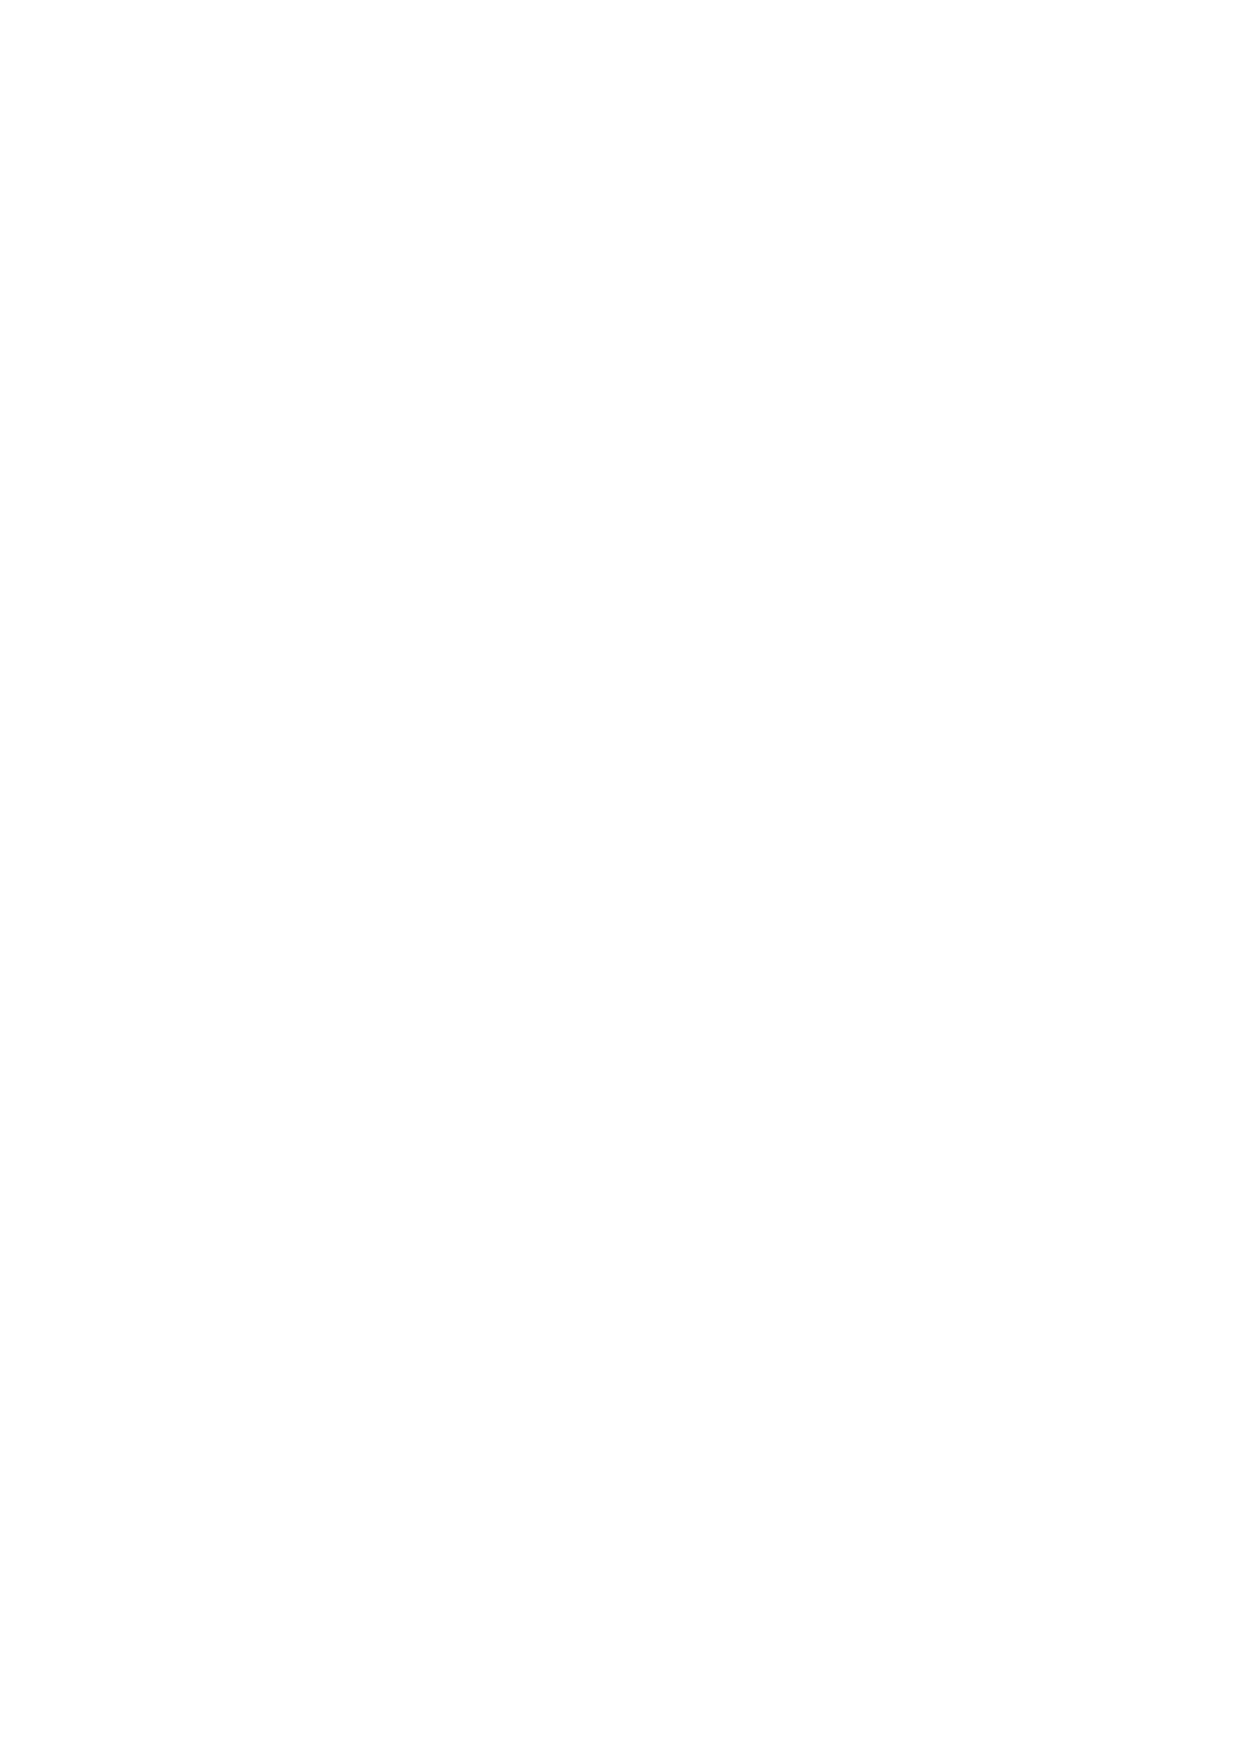
\includegraphics[]{\figs/efficiency} 
\end{figure}

\begin{itemize}
    \item Defining $c$ as a positive integer constant.
    \item For any algorithm, if you find that the complexity is something like $f(n)\leq c\times n^2$ we say that the complexity $O(n^2)$ (Big-O of $n^2$) this is the worse case scenario.
    \item For any algorithm we find that has a complexity of $f(n)\leq c\times n \log_{}\p{ n } $ we say that the algorithm has a worse case scenario of $O(n\log_{}{(n))}$ (Big-O of $n\log_{}\p{ n } $). 
    \item If an algorithm has a complexity of $f(n)\leq c \times 2^n$ (Big-O of $2^n$) this is the worse case scenario.
    \item If however the algorithm is said to have $O(\log_{}\p{ n })$ we understand that the algorithm will never exceed $f(n) \leq c \times \log_{}\p{ n }$ complexity.
    \item Generalizing the concept:  
        \[
            O(g(n)) \qimplies f(n) \leq c \times g(n)
        \]
        \begin{itemize}
            \item Meaning that the algorithm will never take more execution time than $c \times g(n)$, $g(n)$ is any function determined to be the complexity of the algorithm. 
        \end{itemize}
\end{itemize}

\subsection{Example of Big-O}
A function $f(n)$ is said to be $O(g(n))$ if and only if there exists a positive constance $c$ and non negative integer $n_0$ such that $\left| f(n) \right| \leq c \times \left| f(n) \right| $, it is said that $f(n) \in O(f(n))$ 
\begin{figure}[H]
    \centering
    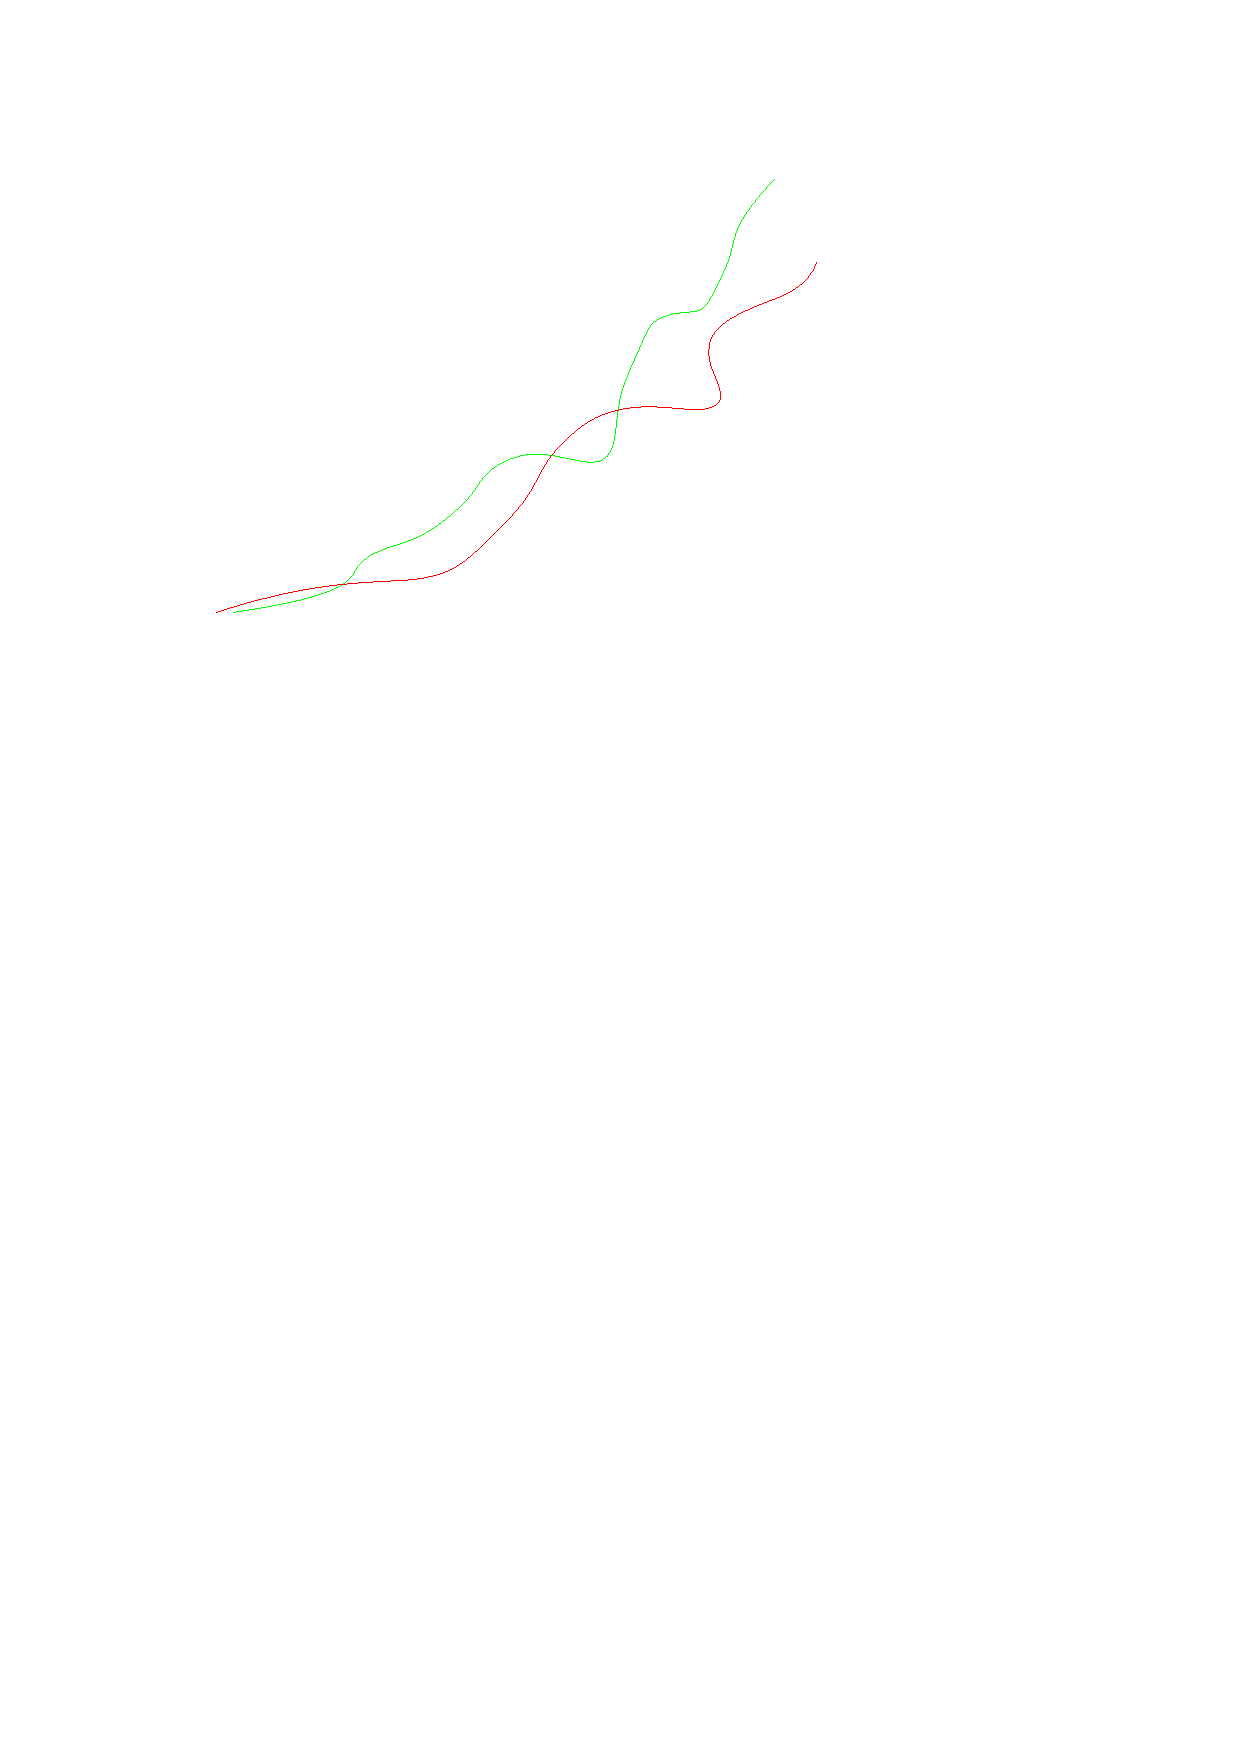
\includegraphics[]{\figs/big-o} 
\end{figure}


%----------------------------------------------------------------------------------------
\section{How to calculate Big-O for a given algorithm}
Before anything lets understand the general polynomial.
\[
  a_k(n) = a_kn^k+a_{k-1}n^{k-1}+\dots+ a_1n+a_0
\]
For any general polynomial we can prove that the value of the polynomial is: 
\[
  \left| a_(n) \right| \leq c \times n ^k, \qq n > n_0
\]
For example, we have the following polynomial:
\begin{center}
   \begin{align*}
       &f(n) = 2n^2+3n+5 \qq \text{ The highest order of $n$ is 2. }\\ 
       &\left| f(n) \right| \leq c \times n^2 \\ 
   \end{align*}
\end{center}
Another example: 
\begin{center}
   \begin{align*}
       &f(n) = 4n^3 + 2n^2 + 3n +7 \\ 
       &\left| f(n) \right| \leq c \times n^3 \\ 
   \end{align*}
\end{center}
If you are given something like this:
\begin{center}
   \begin{align*}
        &f(n) = n\log_{}\p{ n } +n+5 \\ 
        &\left| f(n) \right| \leq c \times n \log_{}\p{ n } \\ 
   \end{align*}
\end{center}
Another example: 
\begin{center}
   \begin{align*}
       &f(n) = 4n +5 \\ 
       &\left| f(n) \right| \leq 4n+n \qq,\; n > 5 \\ 
   \end{align*}
\end{center}

\subsection{Finding Big-O}
We will execute the algorithm using the RAM model hypothetical machine, where each instruction takes a constant amount of time.
\par When finding Big-O you need to account for every instruction, assignments take one unit of time, represented by $c'$, arithmetic operators take one unit of time as well.

\begin{figure}[H]
    \centering
    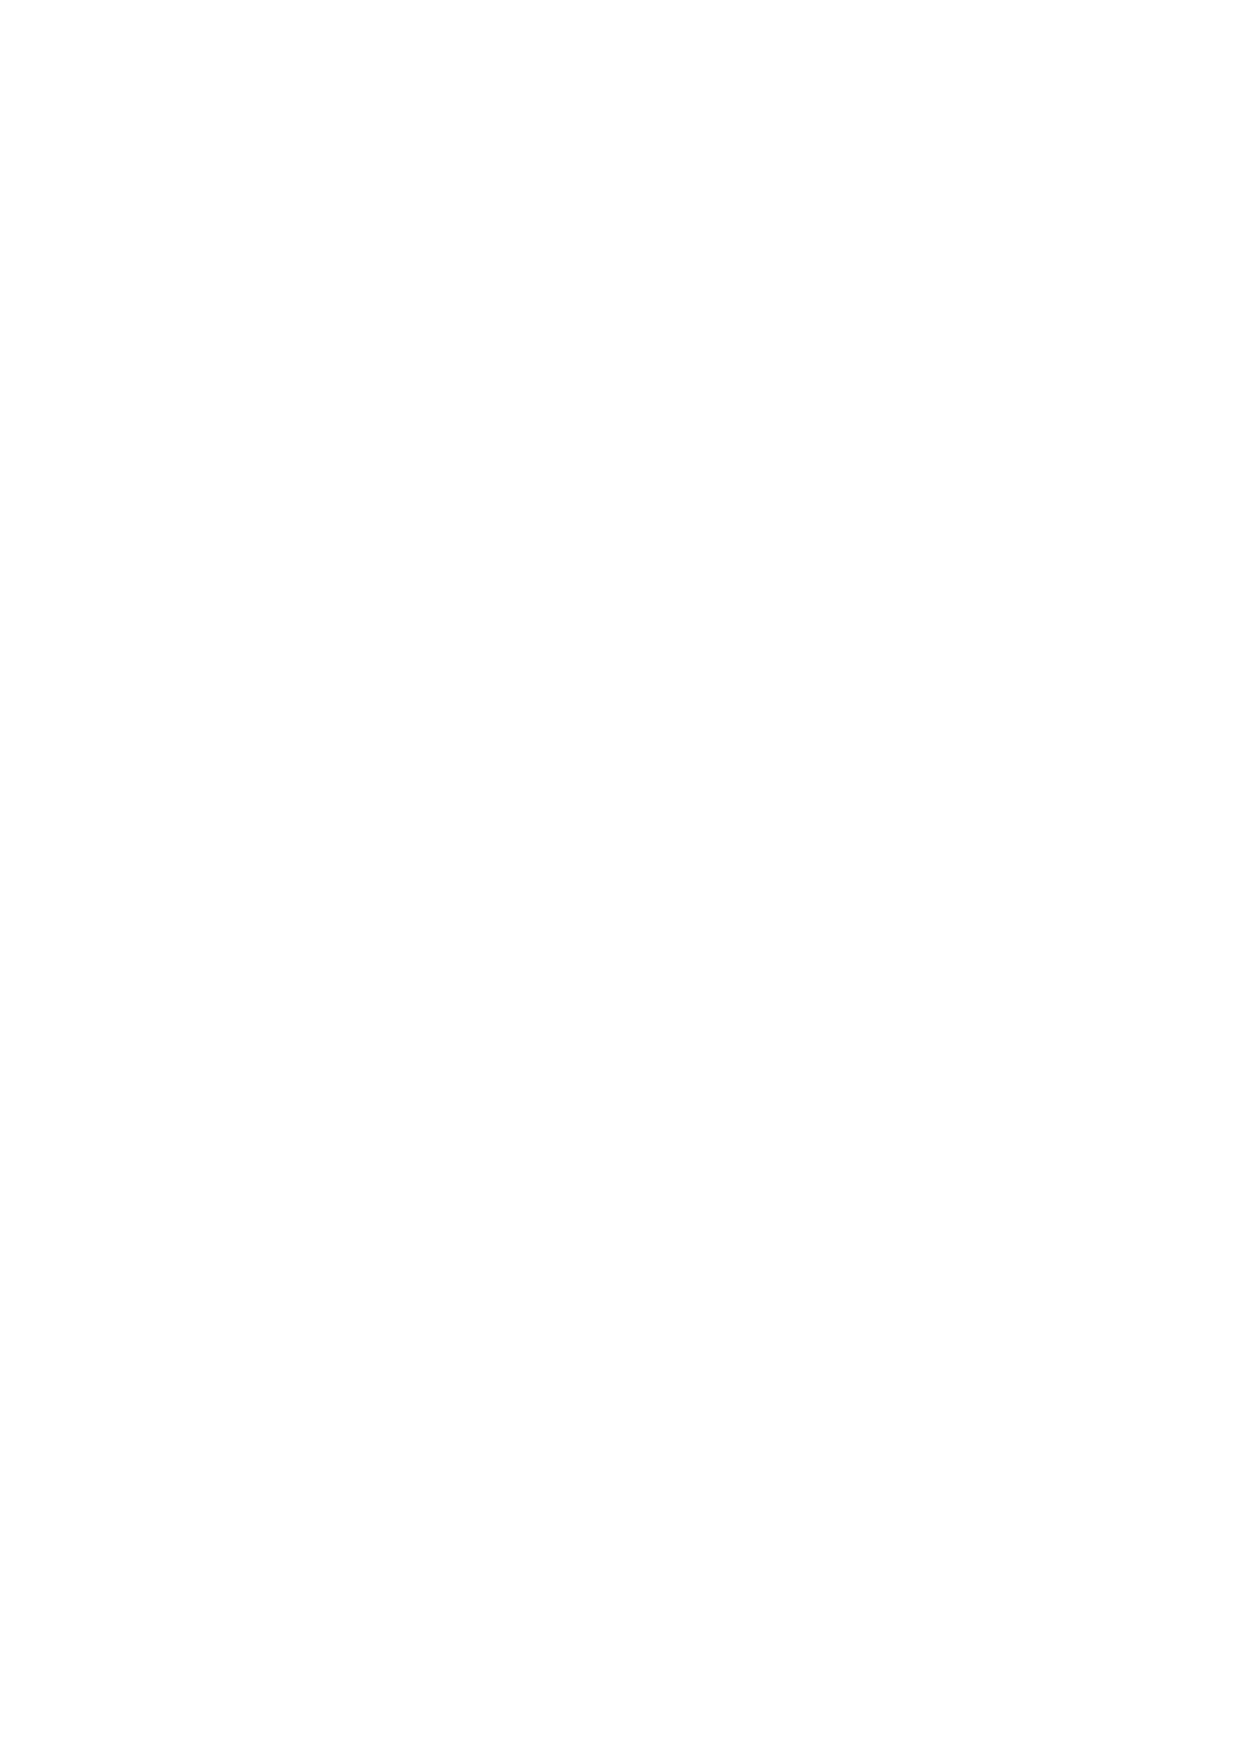
\includegraphics[]{\figs/calculatingbigo} 
\end{figure}
The previous calculation ended in a constant complexity, this means that it doesn't matter the size of the input it will always take the same or constant amount of time to preform the operation. 
The next one, as we can see does not result in constant complexity, it is indeed dependent on the input. 
\begin{figure}[H]
    \centering
    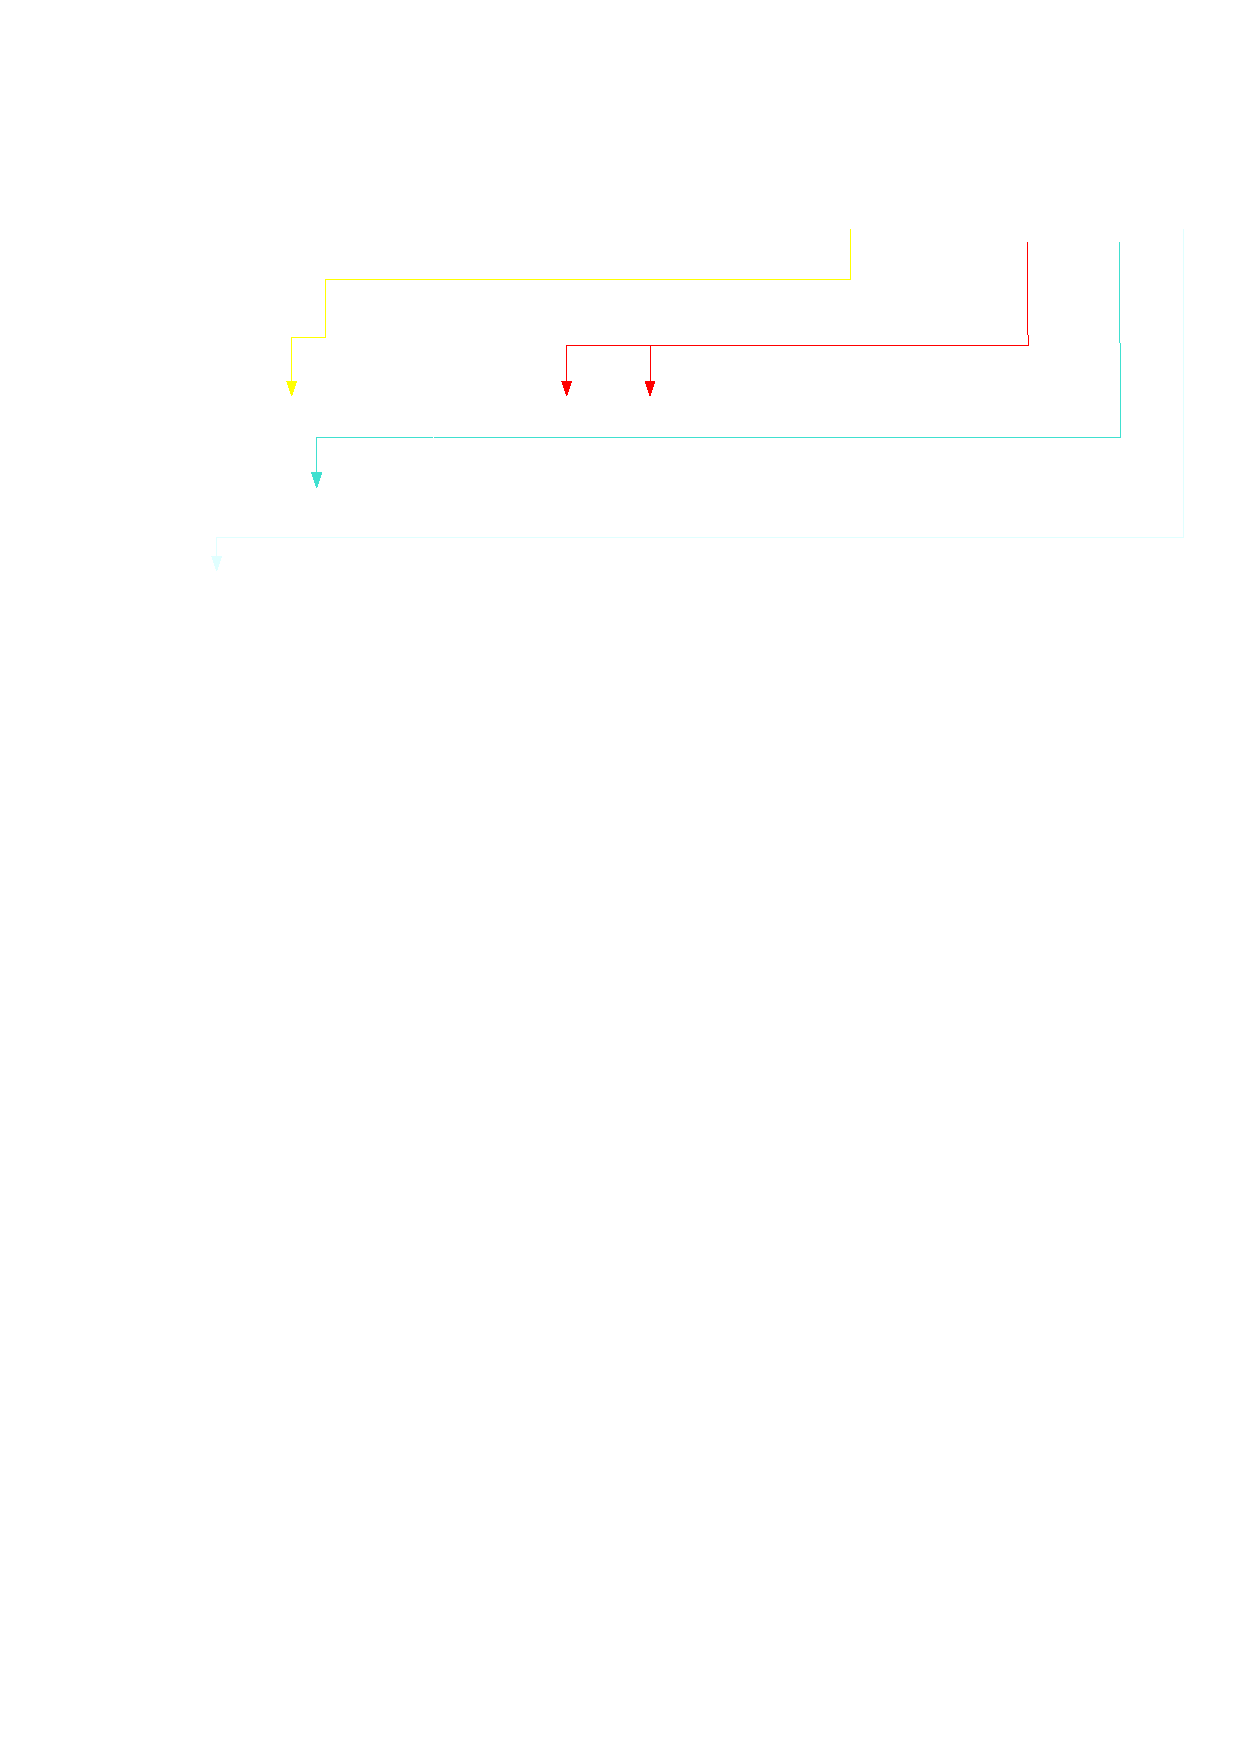
\includegraphics[width=\textwidth]{\figs/calculatingbigo1} 
\end{figure}
As you can see the biggest contributor for the execution time is the for loop. 
\par 
The time taken for is some constant times $n$ thus we can conclude $f(n)\leq O(n)$ which means the complexity is $O(n)$.

\section{Another approach for calculating Big-O - recurrence relationship}
Suppose the same algorithm above, we can find the recurrent relationship which is to say do the following:
\begin{center}
   \begin{align*}
       f(n) &= c + f(n-1)\\ 
       f(n-1) &= c + f(n-2)\\ 
   \end{align*}
   \begin{itemize}
       \item Substitute $f(n-1)$ into $f(n)$ .
   \end{itemize}
   \begin{align*}
        f(n) &= c + (c + f(n-2)) \\ 
        f(n) &= 2c + f(n-2) \\ 
        f(n-2) &= c + f(n-3) \\ 
   \end{align*}
   \begin{itemize}
       \item Do the same and substitute $f(n-2)$ into $f(n)$. 
   \end{itemize}
   \begin{align*}
        f(n) &= 2c + (c + f(n-3)) \\ 
        f(n) &= 3c + f(n-3) \\  
        &\qq \vdots \\ 
        f(n) &= (n-1) * c + f(n-(n-1)) \\ 
        f(n) &= (n-1) * c + f(1) \\ 
        \therefore f(n) &= (n-1) * c + c \\ 
   \end{align*}
\end{center}

\subsection{Another example}
\begin{figure}[H]
    \centering
    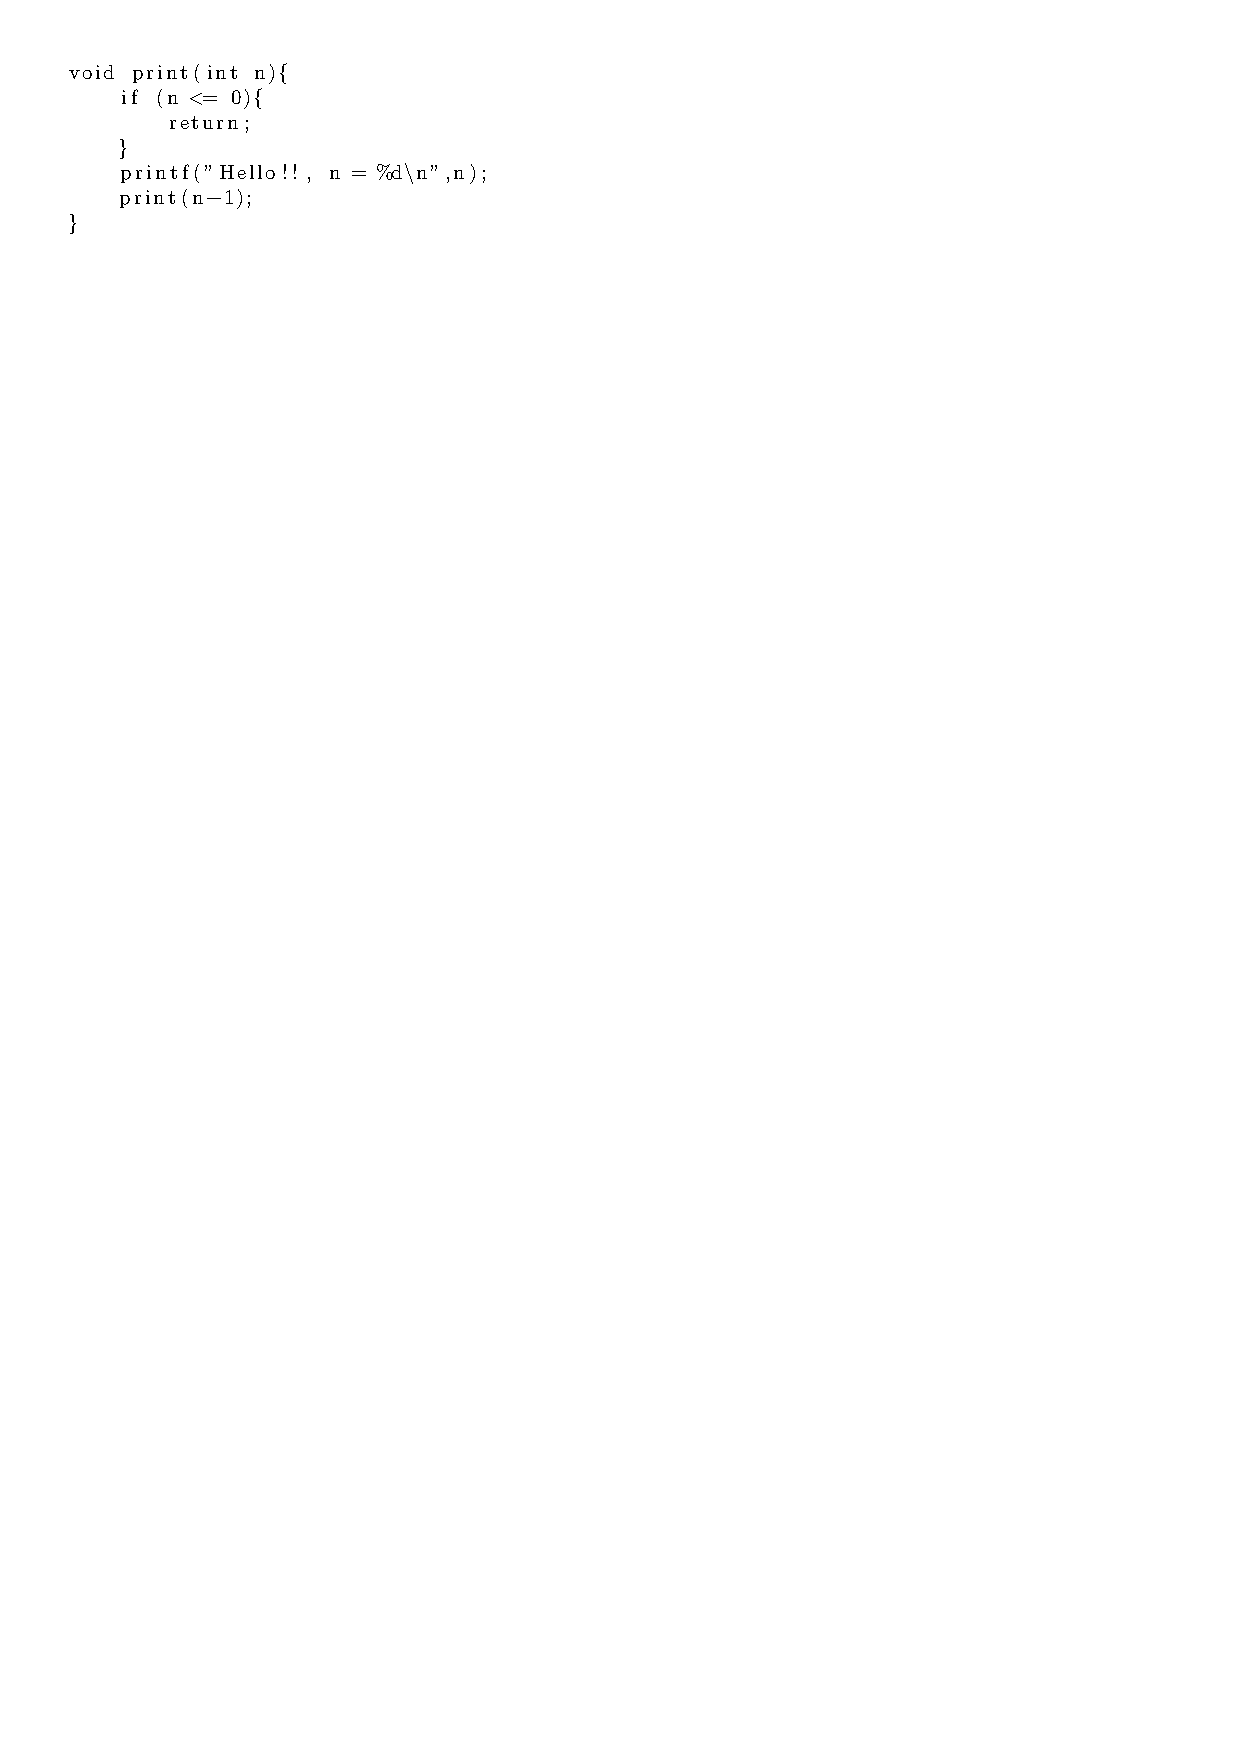
\includegraphics[width=\textwidth]{\figs/bigo2}
\end{figure}

\section{Another example}
\begin{lstlisting}
Algorithm Process (n):
    for (i = n; i >= 1; i = i / 2): 
        < Some simple operations> 
\end{lstlisting}
As you can see, there is a noticeable pattern. 
\begin{center}
   \begin{align*}
       i &= n = \frac{n}{2^0} \\ 
       i &= \frac{n}{2^1} \\ 
       i &= \frac{n}{2^2} \\ 
       &\vdots \\ 
       i &= \frac{n}{n} = \p{\frac{n}{2^k}} \\  
   \end{align*}
   \begin{itemize}
       \item We can find $k$ or the number of times this for loop will repeat.
   \end{itemize}
   \begin{align*}
       \frac{n}{2^k} &= 1 \\ 
       n &= 2^k \\ 
       k &= \log_{2}\p{ n } \\ 
   \end{align*}
\end{center}
Thus the total time taken for this algorithm is: 
\begin{center}
   \begin{align*}
       T &= c \times \log_{2}\p{ n } + c \\ 
       T &= c' \log_{2}\p{ n } \\ 
   \end{align*}
\end{center}
Thus we can say that the complexity of this algorithm is $O(\log_{}\p{ n })$.

\subsection{The same but evaluated with recurrence}
Suppose the same algorithm presented above (Process (n)). Let's define the function.
\begin{center}
   \begin{align*}
       f(n) &= c + f\p{\frac{n}{2}} \\ 
       f\p{\frac{n}{2}}  &= c + f\p{\frac{n}{2^2}}  \\ 
   \end{align*}
   \begin{itemize}
       \item Substitute $f(n/2)$ into $f(n)$.
   \end{itemize}
   \begin{align*}
        f(n) &= c + c + c \p{\frac{n}{2^2}}  \\ 
        &= 2c + \p{\frac{n}{2^2}}  \\ 
        &\vdots \\ 
        &= kc + \p{\frac{n}{2^k}}  \\ 
        &= \log_{2}\p{ n }\times c + f\p{\frac{n}{2^{\log_{2}\p{ n } }} }  \\ 
        &= \log_{2}\p{ n }\times c + f\p{\frac{n}{n}}  \\ 
        &= \log_{2}\p{ n }\times c + c \\ 
   \end{align*}
   \begin{itemize}
       \item It will iterate as long as it is not 1 or $f(1)$.
       \item We can say now that the complexity of this algorithm is: 
   \end{itemize}
   \begin{align*}
       f(n) &\leq c' \times \log_{2}\p{ n } \\ 
       \therefore &\; O(\log_{}\p{ n }) \\ 
   \end{align*}
\end{center}

%----------------------------------------------------------------------------------------
\section{Idea of best case complexity — Big Omega notation}
\begin{itemize}
    \item Unlike the Big-O analysis, the best case analyzes the minimum amount of time that the algorithm will always take. 
    \item It is important to consider that that minimum time will occur in special cases or depending on the input size. 
    \item Def: A function $f(n)$ is said to be $\Omega(g(n))$ if and only if there exists a positive constant $C$ and a non-negative integer $n_0$ such that: 
        \[
          \left| f(n) \right| \geq C \times g(n), \; \forall \; n \geq n_0  
        \]
    
    \item This minimum time will happen only for special scenarios. 
\end{itemize}
\begin{figure}[H]
    \centering
    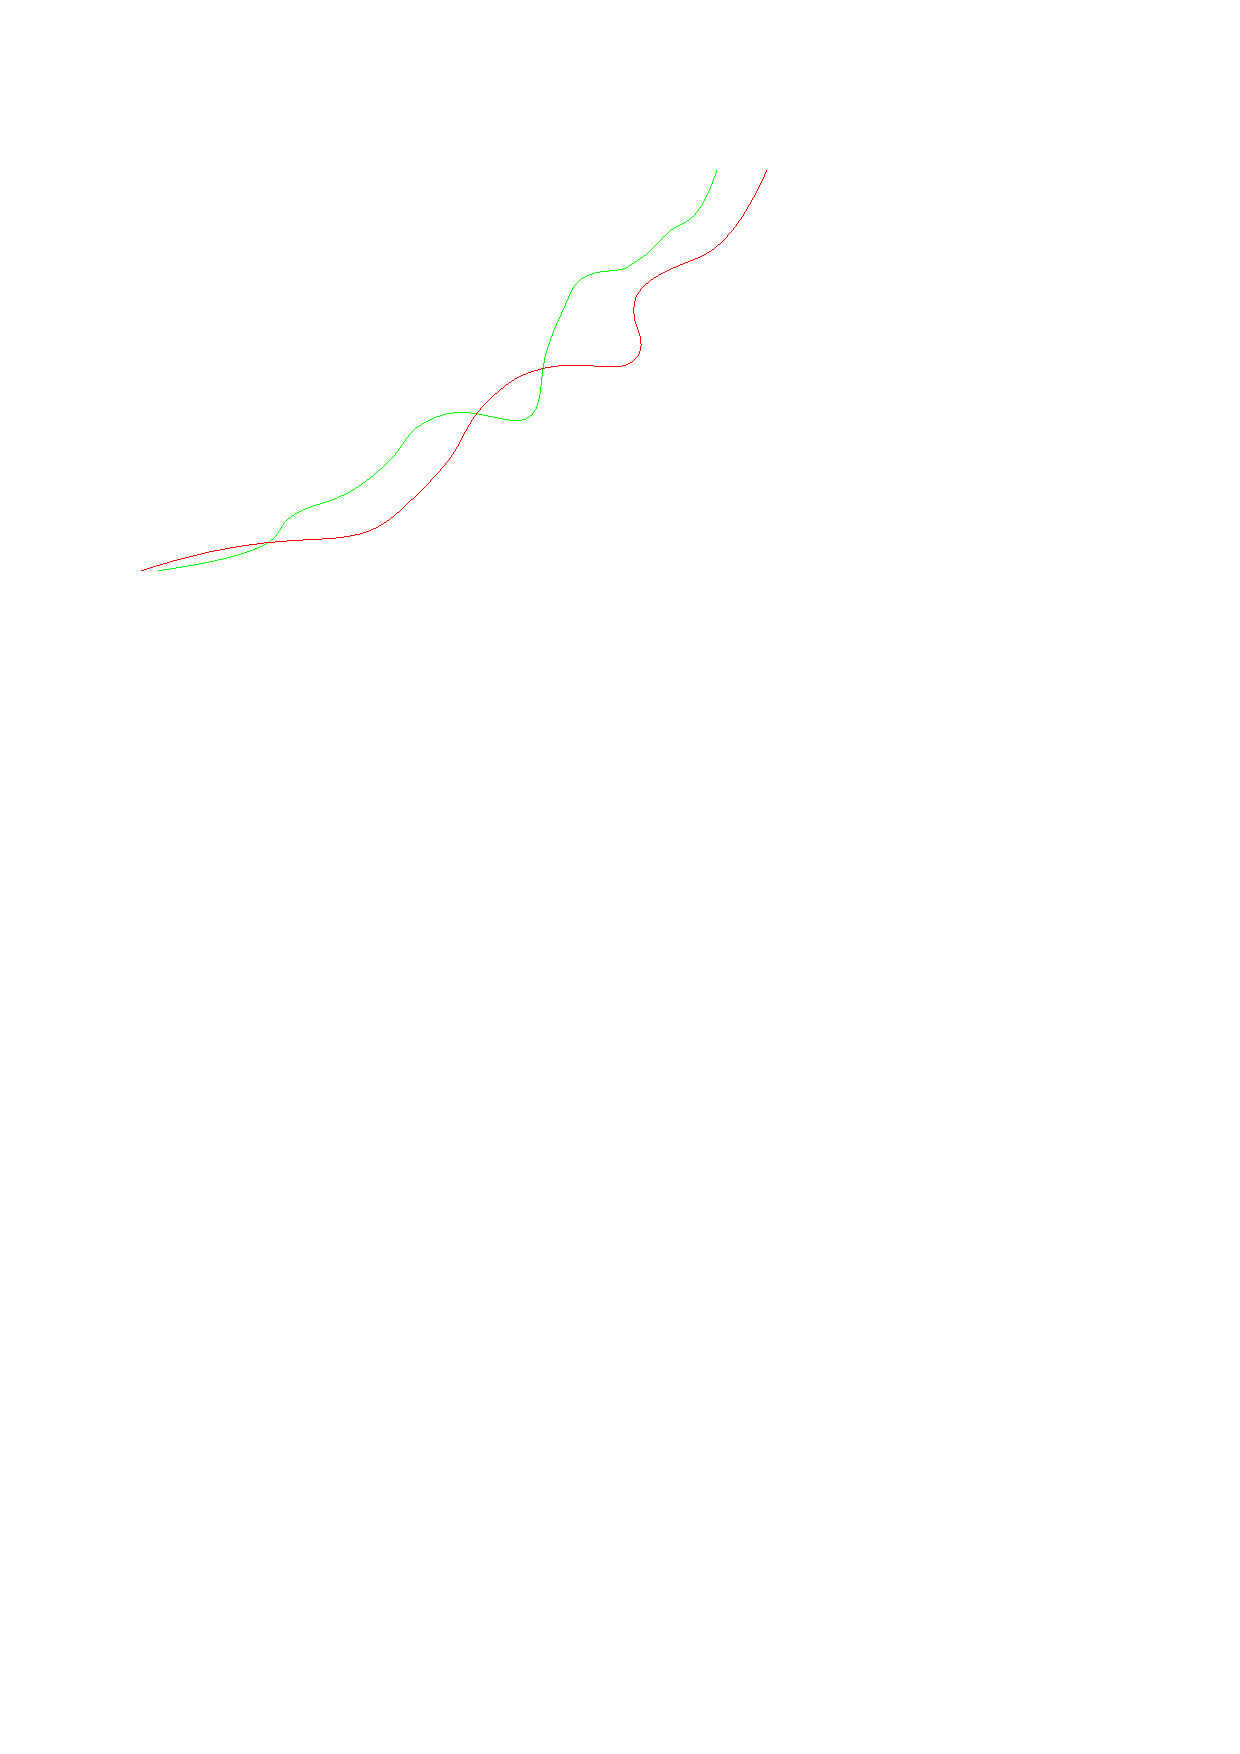
\includegraphics[]{\figs/bigomega} 
\end{figure}

\subsection{Finding Big-$\Omega$ (best case complexity)}
In the following example, searching for 56 is going to require traversing the whole array and returning -1.  The worst case scenario or Big-O, the worst case happens when the item is not found for this algorithm the worst case complexity is $O(n)$.
\begin{figure}[H]
    \centering
    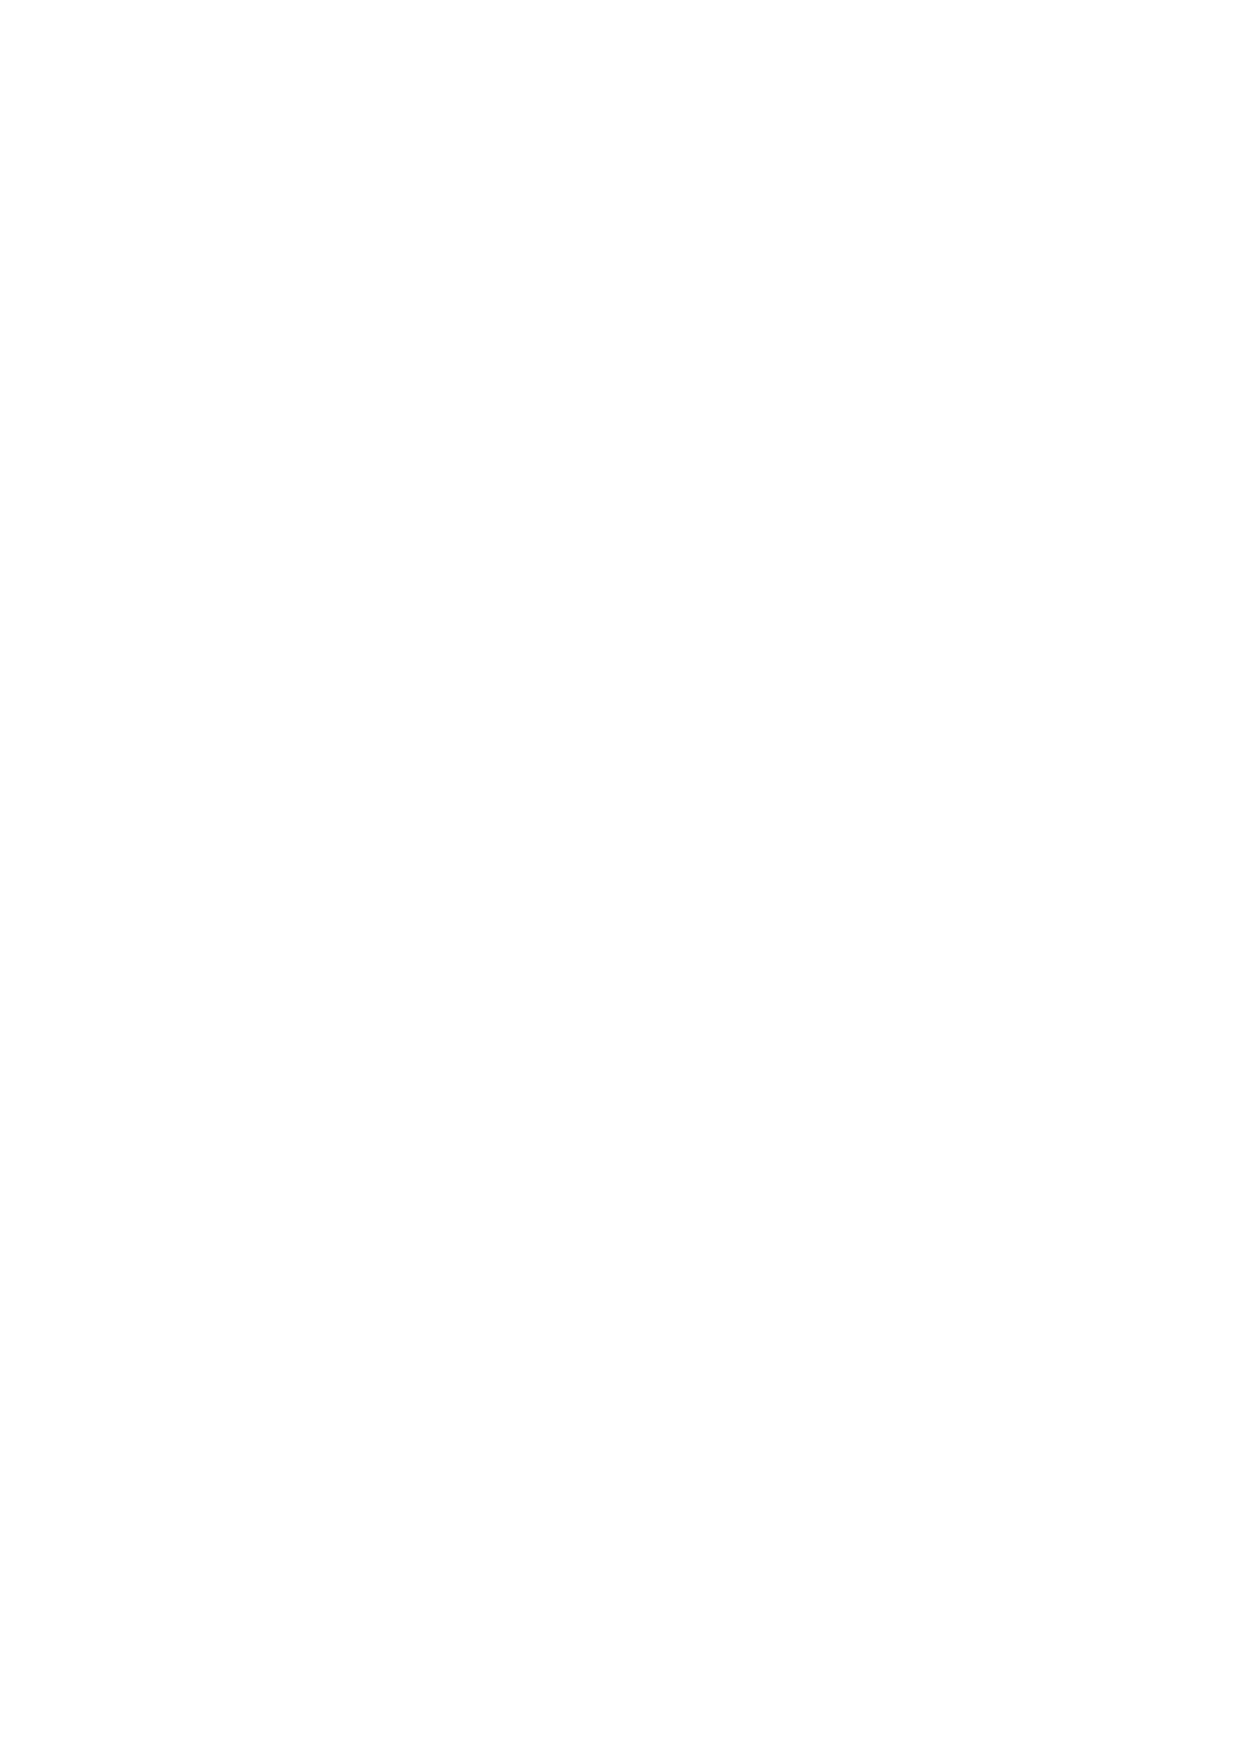
\includegraphics[]{\figs/bigomega1} 
\end{figure}
However, to find 10, in the array, it happens to be the first index, thus we can say that the algorithm's best case complexity is $\Omega(1)$, this is because it takes constant time to find 10, and we assume the best scenario. 

\subsection{An example}
On the following we must find the best case scenario. For this we evaluate the case in which we can take as little amount as possible.
\begin{figure}[H]
    \centering
    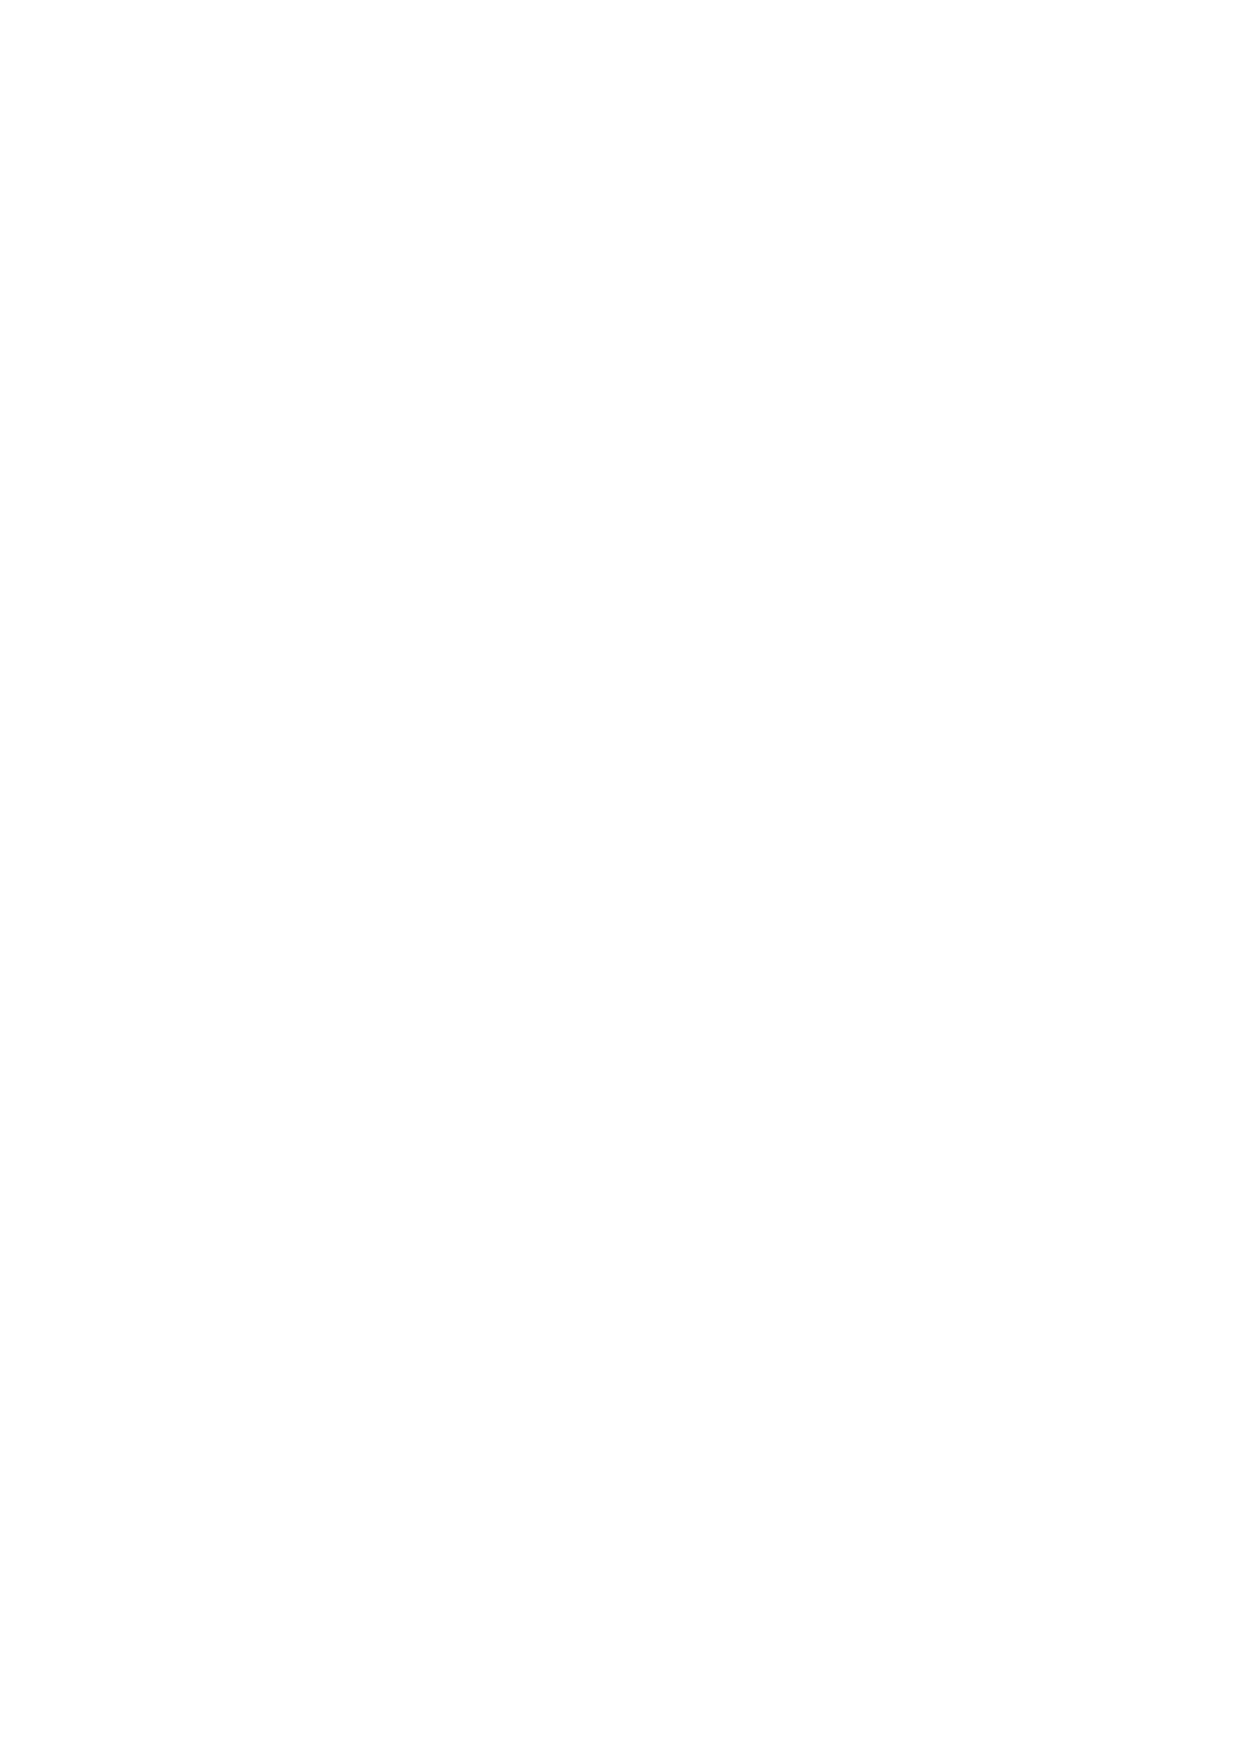
\includegraphics[]{\figs/bigomega2} 
\end{figure}
The worse case complexity is an order of $n^2$ or $O(n^2)$, this is because depending on the variable $k$ the amount of times to iterate is determined, $k$ might never be odd, and this gives us an order of $n^2$. \par 
On the other case, if in the very first iteration $k$ is inputted to be odd, this will break the outer loop condition and make it so that only the inner loop executes $n$ times, this gives us the best case complexity of $\Omega(n)$. 


%----------------------------------------------------------------------------------------
\section{Idea of average case complexity — Big theta notation}
\begin{itemize}
    \item Def. A function $f(n)$ is said to be $\Theta(g(n))$ if and only if there exists two positive constants $C_1$ and $C_2$ and non-negative integer $n_0$ such that:  
        \[
          C_1\times g(n) \leq \left| f(n) \right| \leq C_2, \, \forall \; n \geq n_0
        \]
    
    \item Big-Theta is considered to be more accurate than the others (Big-O and Big-Omega).
\end{itemize}

\begin{figure}[H]
    \centering
    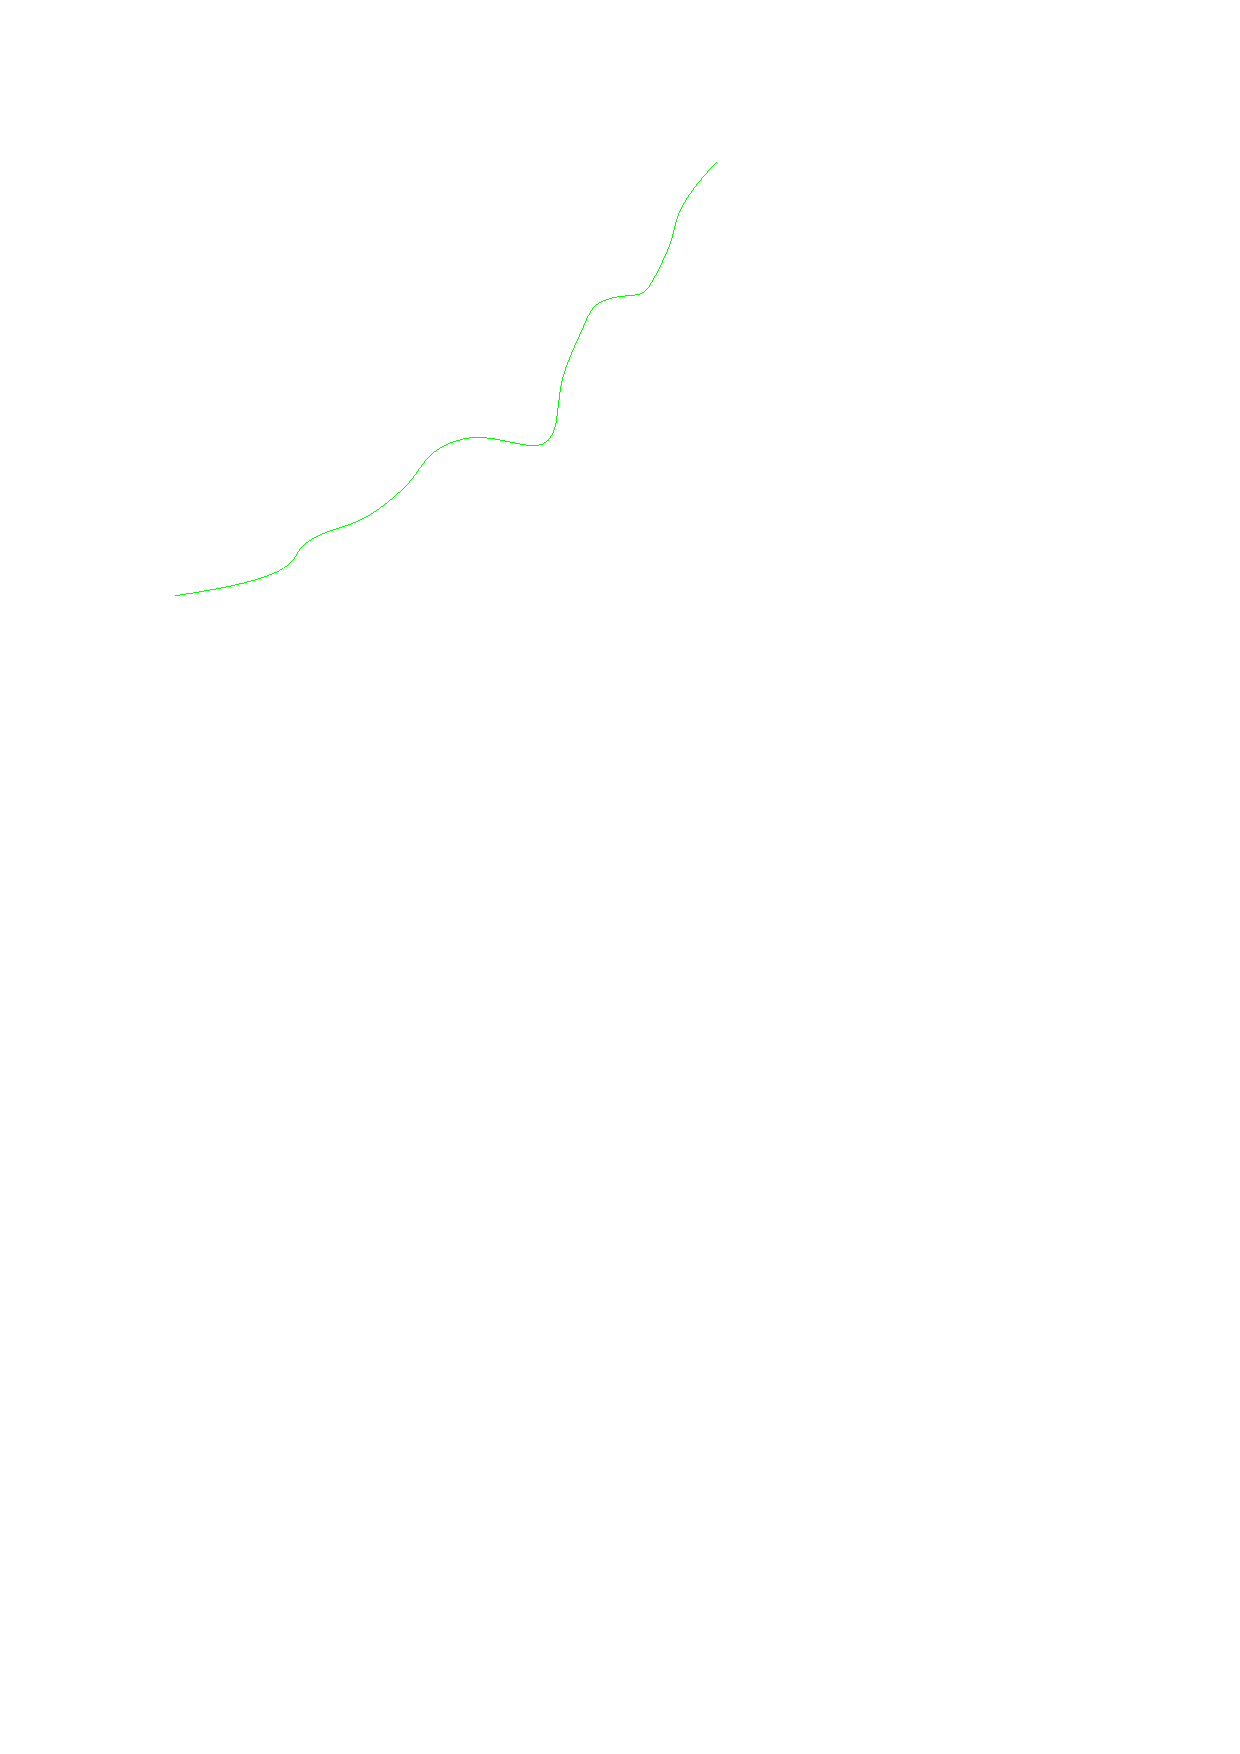
\includegraphics[]{\figs/bigtheta} 
\end{figure}

\subsection{Big theta on polynomials}
\begin{center}
   \begin{align*}
       f(n) &= \frac{1}{2}n^2 - 3n \qq f(n) \in \Theta(n^2) \\ 
       C_1\times n^2 &\leq \frac{1}{2} n^2 - 3n \leq C_2\times n^2 \\ 
   \end{align*}
   \begin{itemize}
       \item Find the inequalities.
   \end{itemize}
   \begin{align*}
        C_1\times n^2 \leq \frac{1}{2} n^2 - 3n, \qq n \geq 12 \\
        C_1 \leq \frac{1}{4}, \qq C_1 = \frac{1}{8} \\ 
        \frac{1}{8} n^2 \leq \frac{1}{2}n^2-3n \\  
   \end{align*}
   \begin{align*}
        \frac{1}{2} n^2 - 3n \leq C_2\times n^2 \\ 
        \frac{1}{2} - \frac{3}{n} \leq C_2 \qq  \qq n \geq 12 \\ 
        \frac{1}{2} - \frac{3}{12} \leq C_2  \\ 
        \frac{1}{2} - \frac{1}{4} \leq C_2 \\ 
        C_2 = 1 \qq C_2 = 2\\  
        \frac{1}{8} n^2 \leq \frac{1}{2} n^2 - 3n \leq n^2 \\ 
        f(n) \in \Theta(n^2) \;\forall \; n \geq 12 \\ 
   \end{align*}
\end{center}
